\section{Approach}
\label{sec:approach}

Figure \ref{fig:architecture_overview} depicts the high-level processes of
\venera that execute when an integrated project is built. There are three
major phases:

\textbf{Analysis.} Test run history is analysed and the probability of failure
for each test is calculated.

\textbf{Instrumentation.} \venera extracts the packaged application, examines
its bytecode and injects state-monitoring probes. Probe placement is informed by
available historical data and is performed with respect to a budget. Tests
determined to be \flaky are prioritised and are more heavily instrumented.

\textbf{Testing.} The test suite is run on the instrumented application; probes
fire events which are processed and logged to files. Logs are stored in a
database along with the test results after completion.

We first define our notion of budget (Section \ref{sec:sec:budget}). Then, we
present a criteria for ranking \flaky tests (Section \ref{sec:sec:flakiness}) so
that budget may be allocated intelligently. Finally, we detail algorithms that
can be used to allocate budget to tests in a suite (Section
{\ref{sec:sec:allocating_budget}).

\begin{figure}[h]

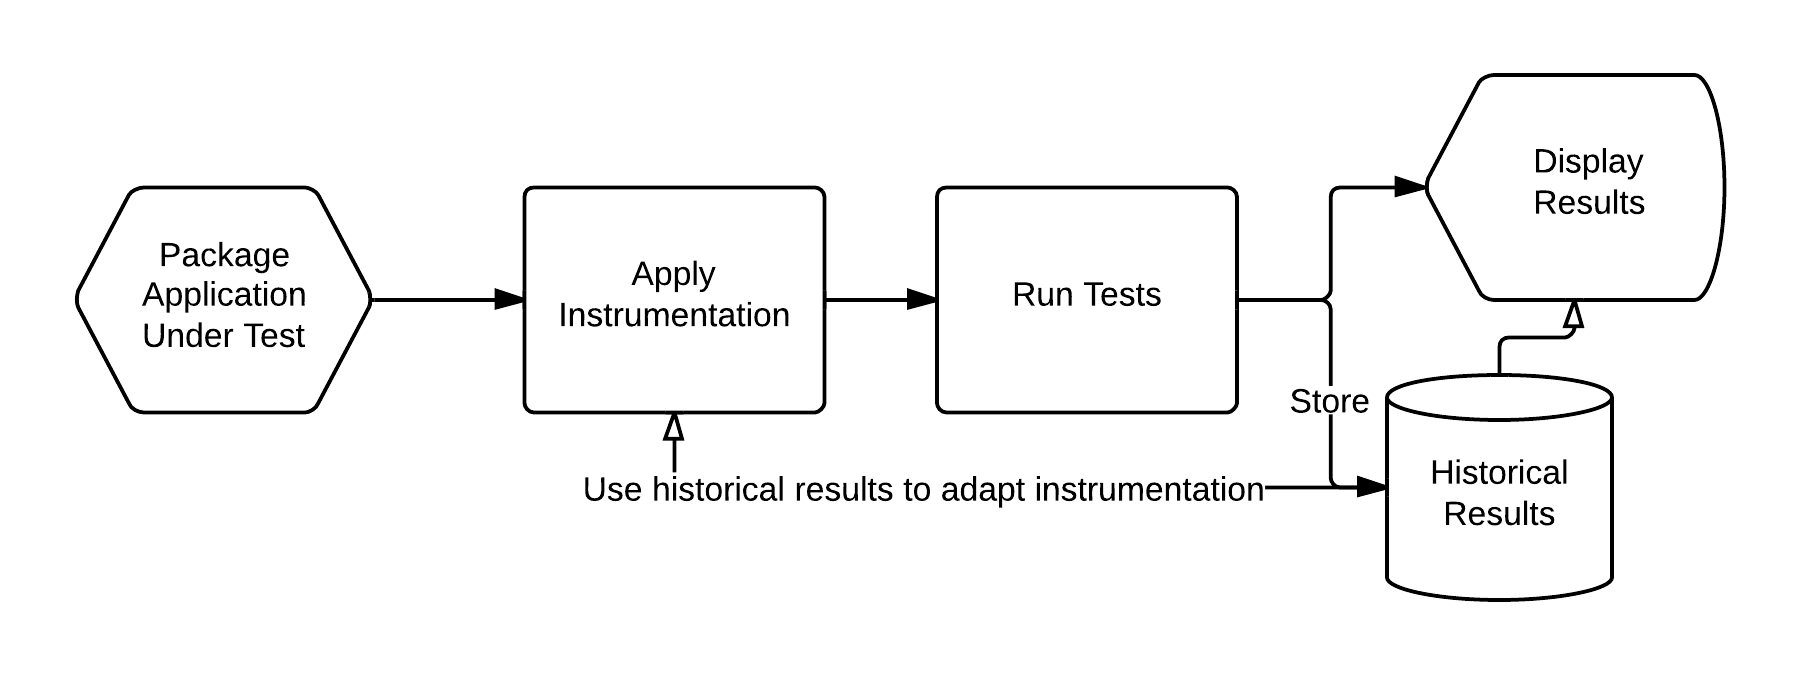
\includegraphics[width=\linewidth]{Images/architecture_overview}

\caption{}
\label{fig:architecture_overview}
\end{figure}


\subsection{Flakiness}
\label{sec:sec:flakiness}

\Flaky tests with a relatively low probability of failure are harder to
reproduce. We define a normalised scalar value --- \emph{\flakiness} (Definition
\ref{def:flakiness}) --- based on probability of test failure. We favour tests
with high \flakiness and instrument them more heavily by assigning \flaky budget
proportionally to \flakiness; Section \ref{sec:sec:allocating_budget} describes
the process in detail. Algorithm \ref{alg:calculate_flakiness} presents a
possible method of calculating \flakiness. It is important to note that
\flakiness is purely a prioritisation-related value --- we could of course
simply divide the \flaky budget equally between all \flaky tests.

\begin{defn}[\Flakiness]
\label{def:flakiness}

Given a test $T$ with probability of failure $T_{p}$, test \flakiness is
calculated by
\begin{align*}
  f(T_{p})=
	\begin{cases}
	    1 - \frac{T_{p}}{\alpha},& \text{if } T_{p}< \alpha\\
	    0,              & \text{otherwise}
	\end{cases}
\end{align*}
where $\alpha$ is the \flaky test threshold; \ie, the point at which $\epsilon$
(as defined in Definition \ref{def:flaky_test}) becomes significant.

\end{defn}

\begin{algorithm}[h]
\caption{}
\label{alg:calculate_flakiness}

\begin{algorithmic}
	\Require{$probOfFailure$ and $threshold$ are decimal values within ranges
	$[0..1]$ and $(0..1]$ respectively.}
    \Statex

	\Function{calculateFlakiness}{$probOfFailure$, $threshold$}

	\If{$(probOfFailure \geq threshold)$ OR $(probOfFailure \eq 0)$}
		\State \Return $0$
	\Else
		\State \Return $1 - (probOfFailure / threshold)$
	\EndIf

	\EndFunction
\end{algorithmic}

\end{algorithm}

\subsection{Test Suite Budget}
\label{sec:sec:budget}

Our budget is time-based. We can calculate the average time to completion for
some test suite $T$ with $\sum\limits_{t \in T} averageTimeToCompletion(t)$.
Given some maximum allowed run time $B^{max}$, we have a test suite budget $B$,
where
\begin{align*}
B = B^{max} - \sum\limits_{t \in T} averageTimeToCompletion(t)
\end{align*}

Note that a sensible value of $B^{max}$ will vary with user needs, so it will be
exposed for modification.


\subsection{Allocating Test Suite Budget}
\label{sec:sec:allocating_budget}

We partition our budget into two pools: \flaky and exploratory. Given our
total test suite budget $B$, we have
\begin{align*}
B = B_{e} + B_{f}
\end{align*}
where $B_{e}$ is the total exploratory budget and $B_{f}$ is the total flaky
test budget.

At the test level, we allocate \flaky budget proportionally to a test's
flakiness. Exploratory budget is uniformly randomly allocated over all tests ---
each test in the suite is equally likely to receive a portion of the exploratory
budget, but not guaranteed.

Given a suite of tests $T$, a test $t \in T$ is allocated budget $B_{t}$, where
\begin{align*}
B_t = \frac{B_f \times T_f}{\sum\limits_{i=1}^{|T|}
f(T_{i_p})} + \frac{B_e}{|T|} + B_{remainder}
\end{align*}
\mc{This is wrong. $B_{remainder}$ is not defined. It \textit{should} be the
remaining budget after the $B_e$ and $B_f$ are allocated. Also $\frac{B_e}{|T|}$
is not how $B_e$ is allocated --- it is allocated over all non-\flaky tests
uniformly until there is no budget remaining. In other words, not all tests will
receive exploratory budget.}

\begin{algorithm}[H]
\caption{Instrumenting the test suite with respect to a budget}
\label{alg:venera}

\begin{algorithmic}
	\Require{$T$ is the set of tests making up the test suite}
	\Require{$B$ is the test suite budget}
	\Require{$proportionFlaky$ is a decimal value in the range $[0..1]$}
	\Statex

	\Function{venera}{$T$, $proportionFlaky$}

	\Statex

	\State allocateBudget($T$, $B$, $proportionFlaky$)
	\Statex

	\ForAll {$t \in T$}
		\State{instrument($t$)}
	\EndFor

	\EndFunction

	\Statex

	\Function{allocateBudget}{$T$, $B$, $proportionFlaky$}

	\State{$flakyBudget \gets B * proportionFlaky$}
	\State{$exploratoryBudget \gets B * (1 - proportionFlaky)$}
	\Statex

	\State{allocateFlakyBudget($T$, $flakyBudget$)}
	\State{allocateExploratoryBudget($T$, $exploratoryBudget$)}

	\EndFunction
\end{algorithmic}

\end{algorithm}

\mc{$proportionFlaky$ is stupid.}

\algref{alg:venera} defines the two main steps: allocation and instrumentation.
First, $B_t$ is calculated for each $t$. Then, the instrumentation is performed.
It is during the instrumentation step that the application is actually modified.

\subsubsection{\Flaky Budget Allocation}
\label{sec:sec:flaky_budget_alloc}

\begin{algorithm}[H]
\caption{Allocating flaky budget to tests}
\label{alg:allocateFlakyBudget}

\begin{algorithmic}
	\Require{$T$ is the set of tests making up the test suite}
	\Require{$B_f$ is the total \flaky test budget}
	\Require{$B_{f}^{max}$ is the maximum \flaky budget for a test}
	\Statex

	\Function{AllocateFlakyBudget}{$T$, $B_f$, $B_{f}^{max}$}

	\State $totalFlakiness \gets 0$

	\For{$t \in T$}
		\State $totalFlakiness \gets totalFlakiness + flakiness(t)$
	\EndFor
	\Statex

	\State $T \gets$ sortByFlakinessDescending($T$)

	\For{$t \in T$}
		\State $B_t \gets$ calculateTestFlakyBudget($t$, $totalFlakiness$, $B_f$,
		$B_{f}^{max}$)
	\EndFor

	\EndFunction
	\Statex

	\Function{calculateTestFlakyBudget}{$t$, $totalFlakiness$, $B_f$,
	$B_{f}^{max}$}

	\State $testFlakyBudget \gets (flakiness(t) / totalFlakiness) * B_f$
	\Statex

	\State \Return minimum($testFlakyBudget$, $B_{f}^{max}$)

	\EndFunction
\end{algorithmic}

\end{algorithm}

\subsubsection{Exploratory Budget Allocation}

Exploratory budget gives us a chance of gathering data from newly flaky tests.

\begin{algorithm}[H]
\caption{Allocating exploratory budget to tests}
\label{alg:allocateExploratoryBudget}

\begin{algorithmic}[1]
	\Require{$T$ is the set of tests making up the test suite}
	\Require{$B_e$ is the total exploratory budget}
	\Require{$B_{e}^{max}$ is the maximum exploratory budget for a test}
	\Statex

	\Function{AllocateExploratoryBudget}{$T$, $B_e$}

	\State KnuthShuffle($T$)
	\State $iterator \gets T.getIterator()$
	\While{$B_e > 0$ AND $iterator.hasNext()$}
		\State $t \gets iterator.getNext()$
		\State \begin{varwidth}[t]{\linewidth}
		$B_e \gets B_e -$\par
		\hskip\algorithmicindent \text{calculateTestExploratoryBudget}($t$,
		$B_e$, $B_{e}^{max}$)
		\end{varwidth}
	\EndWhile

	\EndFunction
	\Statex

	\Function{CalculateTestExploratoryBudget}{$t$, $B_e$, $B_{e}^{max}$}

	\If{$B_t > 0$}
		\Return $0$
	\EndIf

	\State $B_t \gets$ minimum($B_e$, $B_{e}^{max}$)

	\State \Return $B_t$

	\EndFunction
\end{algorithmic}

\end{algorithm}


\subsection{Instrumentation}

\algref{alg:instrument_test} details the basic process for instrumenting a test
with respect to a given budget. {\tt GetNextSetInstrumentationPoints()} returns
a list of instrumentation points ordered by descending priority. An ideal
implementation of the function would take into account previous probe
allocations, test outcomes and budgets.

\begin{algorithm}[H]
\caption{Instrument a test with respect its allocated budget}
\label{alg:instrument_test}

\begin{algorithmic}
	\Require{$t$ is a test}
	\Statex

	\Function{Instrument}{$t$}

	\State{$sites \gets GetNextSetInstrumentationPoints()$}
	\While{$B_t > 0$}
		\ForAll{$site \in sites$}
			\State{$cost \gets site.cost$}
			\If{$cost \le B_t$}
				\State{$site.active \gets true$}
				\State{$B_t \gets B_t - cost$}
			\Else
				% Need to work out how to define new algorithmic-style macros (e.g.
				% \BREAK)
				\State{\textbf{break}}
			\EndIf
		\EndFor
	\EndWhile

	\EndFunction
\end{algorithmic}

\end{algorithm}


\subsection{Monitoring Application State with Probes}
\label{sec:probes}

There are a number of types of points at which it is useful to gather
information about application state. We extend the common approach of counters
and predicates[] to include instrumentation designed for to gather much more
contextual information.

We refer to a piece of code inserted at an instrumentation site to monitor
application state as a probe. Complex probes record the state of live objects
such as variables and method parameters, but carry a large performance overhead.
Predicate probes are a lightweight alternative to monitor execution flow.

Probes are allocated based on the available budget, historical results and
available instrumentation sites. For example, predicate probes could be used to
hone in on program flows associated with failure during initial runs. Later,
once areas of problematic code are identified, heavier-weight complex probes
could then be inserted to gather more detailed information.

Complex probes serialize Java objects to JSON with google-gson. Primitives are
boxed to their object representations.

Predicate probes simply maintain a counter that is incremented each time the
predicate is observed to be true.

\begin{center}
    \begin{tabular}{| l | p{6cm} |}
    \hline
        \textbf{Program Point} & \textbf{Description} \\
    \hline
        \multicolumn{2}{|c|}{\textit{Complex Probes}} \\
    \hline
        Function Entry &
        At the beginning of each function, we serialize all parameter objects
        (boxing primitives), along with all live variables. \\
    \hline
        Function Return &
        At each function call with a return value, we serialize its object
        result. \\
    \hline
        Conditional Branch &
        At each branch point, we record all variables in scope separately for
        each path. \\
    \hline
        Variable Assignment &
        For an assignment $V = E$, where $E$ is an expression, we record both
        the current value of $V$ and the new value of $V$ after assignment. \\
    \hline
        \multicolumn{2}{|c|}{\textit{Predicate Probes}} \\
    \hline
        Conditional Branch &
        At each path of the branch we maintain a counter that is incremented
        every time the path is taken. \\
    \hline

    \end{tabular}
\end{center}

\subsubsection{Probe Cost}
\label{sec:sec:probe_cost}

In order to meet our budget, it is important that we are able to estimate the
effects individual probes have on timing. If our instrumentation causes a
individual test to run over budget, we risk running over budget at the suite
level. We refine probe costs by comparing expected overhead to measured
overhead.

To measure the effects of both the Complex and Simple Method Entry Probes, we
wrote and ran 12 tests. Each of the tests call an empty method with one or more
arguments 100 times. The tests were annotated with {\tt COMPLEX}, {\tt SIMPLE}
and {\tt NONE} policy types. The uninstrumented (\ie, {\tt NONE}) test is used
as a baseline. \autoref{lst:uninstrumented_test} shows the basic structure of
the uninstrumented test with 1 argument --- the others similar. Timings were
measured for the method calls only; start up and shutdown times were ignored.
The tests were run on a Nexus 5 running Android version 4.2.2.

\begin{lstlisting}[caption=Uninstrumented Test,label=lst:uninstrumented_test]
@Venera(instrumentationPolicy = NONE)
public void testUninstrumentedEmptyMethod() {
	Stopwatch.createStarted();
	for (int i = 0; i < 100; i++) {
		anUninstrumentedEmptyMethod(i);
	}
	Stopwatch.stop();
}

@Venera(instrumentationPolicy = NONE)
private void anUninstrumentedEmptyMethod(int unusedParameter) {
}
\end{lstlisting}

\begin{figure}[h]

\centering
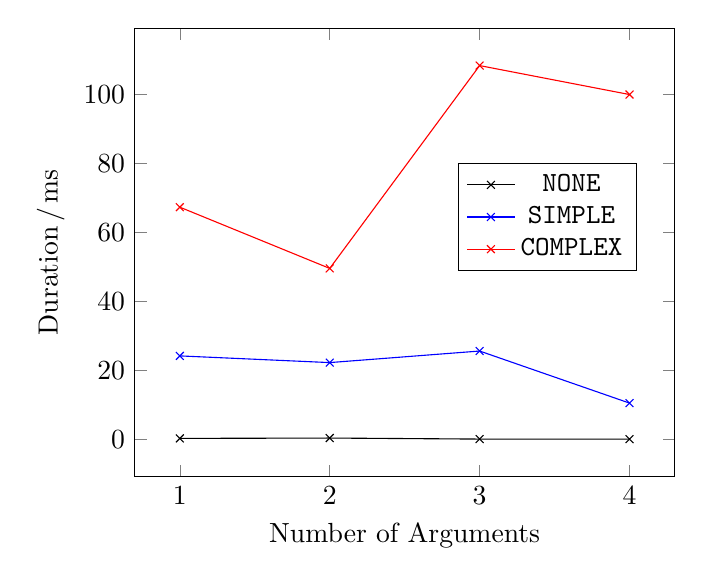
\begin{tikzpicture}
	\begin{axis}[
		xlabel = Number of Arguments,
		ylabel = Duration\,/\,ms,
		xtick={1, 2, 3, 4},
		legend style = { at = {(0.93,0.7)} },
	]
		\addplot[
			color = black,
			mark = x,
		] coordinates {
		( 1, 0.2626 )
		( 2, 0.3652 )
		( 3, 0.0645 )
		( 4, 0.0364 )
		};
		\addlegendentry{\tt NONE} ;
		\addplot[
			color = blue,
			mark = x,
		] coordinates {
		( 1, 24.17 )
		( 2, 22.23 )
		( 3, 25.58 )
		( 4, 10.49 )
		};
		\addlegendentry{\tt SIMPLE} ;
		\addplot[
			color = red,
			mark = x,
		] coordinates {
		( 1, 67.27 )
		( 2, 49.52 )
		( 3, 108.3 )
		( 4, 99.91 )
		};
		\addlegendentry{\tt COMPLEX} ;
	\end{axis}
\end{tikzpicture}

\caption{}
\label{fig:test_perf_results}
\end{figure}

With the initial results from the performance tests
(\autoref{fig:test_perf_results}), we can expect that a Complex Instance Method
Entry probe will have an associated overhead of approximately 250 times that of
the original method call, with a Simple Instance Method Entry probe having less
at roughly 60.

Our collected data is not ideal. Each of the data points is backed by only one
measured value and it is clear that the Android platform has intefered with
the results. In order to properly evaluate the cost of our probes, we will need
to measure a large number of methods over multiple runs to smooth out the data.

In the case of Complex Instance Method Entry probes, we would expect an increase
in overhead as a function of the number of parameters of the instrumented
instance method. To a certain extent, the data shows that it is indeed the case,
but it is impossible to be sure with so few data points.

\subsection{Instrumentation Points}
\label{sec:sec:instrumentation_points}

There are potentially millions of lines of code, where do we place our
instrumentation?

Given an entry point, in our case, a test or setup method, we simply take the
next set of code units in the control flow graph.

The main strategy is to place probes further and further down the control
dependence graph until we are able to detect a failure-predicting predicate.

Once we have detected a failure-predicting predicate, we can assign the majority
of our budget to drill down in related areas. Still, we reserve a portion to
‘scout’ in case we get lucky and find another failure predicting predicate
elsewhere.


\subsection{Countering the {\lq}Observer Effect{\rq}}
\label{sec:sec:observer_effect}

If our instrumentation happens to perturb the behaviour of a \flaky test in such
a way that $\epsilon$ is observed to have changed, we reduce the budget
allocated to the test until $\epsilon$ returns to its previous value.
